\documentclass[12pt]{article}
\usepackage{amsmath,amssymb,amsthm}
\usepackage{mathrsfs}
\usepackage{algorithmic}
\usepackage{verbatim}
\usepackage{graphicx}
\usepackage{latexsym}
\usepackage{euscript}
\usepackage{vmargin}
\usepackage[dvips]{epsfig}
\usepackage{pst-tree}
\usepackage{psfrag}
%\usepackage{flafter}%that's only to keep figures from floating
%\usepackage{natbib} %DOES NOT WORK

%\usepackage{notebook2e}
%\usepackage{lcaption}

\setpapersize{USletter}
\setmarginsrb{2.5cm}{2.5cm}{2.5cm}{1.75cm}{0pt}{0mm}{0pt}{0.70cm}

%Array
\setlength{\tabcolsep}{30pt}
\renewcommand{\arraystretch}{1.2}

% Lcaption
%\smartcap
%\CapSize=4.5in


% Float Control
\renewcommand{\topfraction}{0.95}
\renewcommand{\bottomfraction}{0.95}
\renewcommand{\textfraction}{0.05}
\renewcommand{\floatpagefraction}{.95}


%\title
%{set up}
%\author{}

\begin{document}
\bibliographystyle{plain}
%\maketitle
%\begin{abstract}
%\end{abstract}
%\include{bellman_is}
%\section{Ratios of normalizing constants}
In the first subsection, we assume that the pseudo--data points have been determined and explain how to estimate the expectations of interest for a particular $(m_1,m_2)$. 

Let $\mathbf{y}_1=\mathbf{y}_{i}^{m_1}$, $\mathbf{y}_2=\mathbf{y}_{i+1}^{m_2}$, $\mathbf{y}_3=(\mathbf{y}_{i}^{m_1},\mathbf{y}_{i+1}^{m_2})$. We denote the likelihood densities $L_{l}(\xi)=p(\mathbf{y}_l|\xi),l=1,2,3$ and the posterior densities $p_l(\xi)=p(\xi|\mathbf{y}_l),l=0,\ldots,3$. Let $\zeta_0$ and $q_0(.)$ denote the normalizing constant and unnormalized density, respectively, for the prior i.e. $p_0(\xi)=q_0(\xi)/\zeta_0$. Let $\zeta_l=p(\mathbf{y}_l)=\mathrm{E}[L_l(\xi)],l=1,2,3$. We denote the un--normalized posterior densities $q_l(\xi),l=1,2,3$ i.e. $p_l(\xi)=p_0(\xi)L_l(\xi)/\zeta_l=q_l(\xi)/(\zeta_0\zeta_l),l=1,2,3$.
%We assume that the likelihoods $L_l(.)$ are known exactly i.e. that there are no unknown normalizing constant depending on $\xi$ (see Gelman et al, 2004, Section 10.4 for counterexamples). 

By assumption, each of $\mathbf{y}_l,l=1,2,3$ is associated with a known pseudo data point $\mathbf{y}_l^*,l=1,2,3$. The same conventions apply, with the addition of superscript $^*$. In addition, let $\pi_{l}(.)$ denote a completely known approximation to $p_l^*(.)$ for $l=0,\ldots,3$ (see Gelman et al, 2004, Chapter 9). This can be complemented with an adative procedure as in Oh and Berger, 1992. 

Our problem is to estimate
\begin{align}
r=\frac{\zeta_{3}}{\zeta_{1} \zeta_{2}}
\end{align}under the constraint that, we can only use knowledge of $p_l^*(.),l=1,2,3$ for constructing importance distributions and generate samples from them. 

For the standard ratio of normalizing constant problem say $\zeta_1/\zeta_2$, a number of related methods are available: importance sampling (IS), bridge sampling (BS), path sampling (PS), ratio importance sampling (RIS) and linked importance sampling (LIS). See Gelman and Meng, 1997 for the first three, Chen and Shao, 1997 for the fourth, and Neal, 2005 for the last one. A summary of the first four is provided by Chen et al., 2000. IS, BS and RIS are both conceptually and practically simpler than the other two which were developed to address challenging cases. 

We define the relative error as
\begin{align}
\mathrm{RE}^2(\hat r)=\mathrm{E}[(\hat r-r)^2]/r^2
\end{align}

\subsection{IS}
Observe that 
$\mathrm{E}_{\pi_l}[q_l(\xi)/\pi_l(\xi)]=\zeta_0\zeta_l$ and therefore
\begin{align}\label{r_is}
r_{\mathrm{IS}}=\frac{\mathrm{E}_{\pi_0}[q_{0}(\xi)/\pi_0(\xi)]\mathrm{E}_{\pi_3}[q_{3}(\xi)/\pi_3(\xi)]}{\mathrm{E}_{\pi_1}[q_{1}(\xi)/\pi_1(\xi)]\mathrm{E}_{\pi_2}[q_{2}(\xi)/\pi_2(\xi)]}
\end{align}By estimating the expectations above by iid draws from the $\pi_l$'s the relative error is, by the delta method,
\begin{align}
\mathrm{RE}^2= \sum_{l=0}^3\frac{1}{n_l^*}\mathrm{E}_{\pi_l}[\left(\frac{p_{l}(\xi)-{\pi}_l(\xi)}{{\pi}_l(\xi)}\right)^2]+o(1/n_*)
\end{align}
%&=\sum_{l=0}^3\frac{\mathrm{V}_{\pi_l}[q_{l}(\xi)]}{n_l c_l^2}+o(1/n)\\
%&=\sum_{l=0}^3\frac{1}{n_l}\mathrm{E}_{\pi_l}[\left(\frac{p_{l}(\xi)-{\pi}_l(\xi)}{{\pi}_l(\xi)}\right)^2]}+o(1/n)\\
%&=\sum_{l=0}^3\frac{1}{n_l}\mathrm{E}_{\pi_l}[\left(\frac{(p_{l}(\xi)-p^*_{l}(\xi))-({\pi}_l(\xi)-p^*_{l}(\xi))}{{\pi}_l(\xi)}\right)^2]}+o(1/n)
We now turn to another importance sampling formulation. Define $r^*=\frac{\zeta_{3}^*}{\zeta_{1}^*\zeta_{2}^*}$ and $\tilde r=r/r^*$. From the decomposition $p_l(\xi)=q_0(\xi)L(\mathbf{y}_l|\xi)/(\zeta_0 \zeta_l)$ we see that $\zeta_l/\zeta_l^*=\mathrm{E}_{p_l^*}[L_l(\xi)/L_l^*(\xi)]$ and
\begin{align}
\label{r_tilde_is}
\tilde{r}_{\mathrm{IS}}&=\frac{\mathrm{E}_{p_3^*}[L_{3}(\xi)/L^*_3(\xi)]}{\mathrm{E}_{p_1^*}[L_{1}(\xi)/L^*_1(\xi)]\mathrm{E}_{p_2^*}[L_{2}(\xi)/L^*_2(\xi)]}\\\label{r_star_is}
r^*_{\mathrm{IS}}&=\frac{\mathrm{E}_{p_1^*}[\pi_1(\xi)/q_1^*(\xi)]\mathrm{E}_{p_2^*}[\pi_2(\xi)/q_2^*(\xi)]}{\mathrm{E}_{p_0}[\pi_0(\xi)/q_{0}(\xi)]\mathrm{E}_{p_3^*}[\pi_3(\xi)/q_3^*(\xi)]}
\end{align}Each estimate of the components of $r^*$ will be reused across various combinations $(j,m)$ therefore we can afford to spend large amounts of simulation draws to estimate them. The formulation (\ref{r_tilde_is}) is more appealing than (\ref{r_is}) because it involves only likelihood calculations which are sometimes amenable to approximations that are faster to compute.

%\subsection{Bridge sampling}
%As already noted, the estimator for $(\ref{r_tilde_is_2})$ is convenient. Also, it's performance depends on the variability of $L_l(.)/L_l^*(.)$. Rather than spend resources on finding sampling schemes to correct for the variability of $L_3(.)/L_3^*(.)$, it seems more straightforward to ensure that the latter be kept low in the first place, which is the topic of Section . Therefore, our focus is on an alternative formulation to $(\ref{r_star_is_2})$, for example: 
%\begin{align}
%r^*_{\mathrm{BS}}=\frac{\mathrm{E}_{p_1^*}[L_2^*(\xi)\alpha_1(\xi)]\mathrm{E}_{p_2^*}[L_1^*(\xi)\alpha_2(\xi)]}{\mathrm{E}_{p_0}[L_3^*(\xi)\alpha_1(\xi)]\mathrm{E}_{p_0}[L_3^*(\xi)\alpha_2(\xi)]}
%\end{align}which follows from $p_1^*(\xi)L_2(\xi)\alpha_1(\xi)=\frac{p_0(\xi)L_1^*(\xi)}{\zeta_1}L_2^*(\xi)\alpha_1(\xi)=\frac{\zeta_3}{\zeta_1}\frac{p_0(\xi)L_3^*(\xi)}{\zeta_3}\alpha_1(\xi)=\frac{\zeta_3}{\zeta_1}p_3^*(\xi)\alpha_1(\xi)$.
\subsection{RIS}
We now consider a ratio importance sampling formulation and $p_{1,2}^*(.)$, an arbitrary distribution of the form $p_{1,2}^*(\xi)=p_0(\xi)L_{1,2}(\xi)/\zeta_{1,2}^*$. Define
\begin{align}
\tilde{r}_{\mathrm{R}}=\frac{\mathrm{E}_{p_{1,2}^*}[L_{1}(\xi)L_{2}(\xi)/L_{1}^*(\xi)]}{\mathrm{E}_{p_{1,2}^*}[L_{1}(\xi)/L_{1,2}^*(\xi)]\mathrm{E}_{p_{1,2}^*}[L_{2}(\xi)/L_{1,2}^*(\xi)]}
\end{align}and note that $r=\tilde{r}_{\mathrm{R}}\times \zeta_{1,2}^*$. The advantage of this formulation is that if the same sample $\{\xi^k\}_{k=1}^{k_*}\stackrel{\mathrm{iid}}{\sim} p_{1,2}(\xi)$ is used for estimating each expectation, we can reuse the integrands in the denominator to compute the numerator. The price, however, is that we have to determine the optimal $p_{1,2}^*$ for each combination of clusters $(c_i,c_{i+1})$. Again, this cost can be amortized over all combination of data points $(\mathbf{y}_i^j,\mathbf{y}_{i+1}^m)$ which map to $(c_i,c_{i+1})$.







%\include{data_clustering}
%\include{figures}
%\include{sr}
%\include{fgt_copy}
%\include{specific_models}
\documentclass{article}
\usepackage[
bibencoding=auto
,backend=biber
,sorting=ynt
% ,style=verbose-ibid
% ,citetracker
% ,sorting=none
% ,autolang%error: no value specified for autolang.
]{biblatex}
\usepackage{csquotes, datetime2, keyfloat}
\usepackage{amsmath, amssymb}
%\newcounter{res}
%\newtheorem{result}[res]{Result}
\usepackage{filecontents}
\begin{filecontents*}{\jobname.bib}
@article{Sellke1983,
% @article{10.1093/biomet/70.2.315,
%    author={SELLKE, T. and SIEGMUND, D.},
    author={Sellke, T. and Siegmund, D.},
    title={Sequential analysis of the proportional hazards model},
    journal={Biometrika},
    volume={70},
    number={2},
    pages={315-326},
    year={1983},
    month={08},
    abstract ={For the proportional hazards model of survival analysis, an appropriate large-sample theory is developed for cases of staggered entry and sequential analysis. The principal techniques involve an approximation of the score process by a suitable martingale and a random rescaling of time based on the observed Fisher information. As a result we show that the score process of the partial likelihood and the maximum partial likelihood estimator behave asymptotically like Brownian motion.},
    issn={0006-3444},
    doi={10.1093/biomet/70.2.315},
%    url={https://doi.org/10.1093/biomet/70.2.315},
    eprint={https://academic.oup.com/biomet/article-pdf/70/2/315/632076/70-2-315.pdf},
}
@book{Lawless2002,
  title={Statistical Models and Methods for Lifetime Data, Second Edition},
  author={Lawless, Jerald F.},  
  isbn={9781118033005},
  series={Wiley Series in Probability and Statistics},
  year={2002},
  month={11},
  day={13},
  publisher={Wiley},
  doi={10.1002/9781118033005}
}
@book{ 
Ibrahim2004,
author={Ibrahim, Joseph G. and Chen, Ming-Hui and Sinha, Debajyoti},	
title={Bayesian Survival Analysis},
publisher={Springer},
year={2004},
month={12},
day={07},
isbn={9780387952772}
}
%@book{van1998asymptotic,
@book{Vaart1998asymp,
  title={Asymptotic Statistics},
  author={van der Vaart, Adrianus Willem},
  isbn={9780521496032},
%  lccn={98015176},
  series={Cambridge Series in Statistical and Probabilistic Mathematics, 3},
%  url={https://books.google.com/books?id=udhfQgAACAAJ},
  year={1998},
  publisher={Cambridge University Press}
}
@article { 
Bilias1997,
author={Yannis Bilias and Mingao Gu and Zhiliang Ying},	
title={Towards A General Asymptotic Theory For Cox Model With Staggered Entry},
journal={Annals of Statistics},
volume={25},
number={2},
pages={662--682},
year={1997}
}
@article{ 
1998Carlin,
author={Carlin, Bradley P. and Kadane, Joseph B. and Gelfand, Alan E.},
title={Approaches for Optimal Sequential Decision Analysis in Clinical Trials},
journal={Biometrics},
volume={54},
pages={964--975},
year={1998}
}
@article{ 
1994Jacobson,
author={Jacobson, M.A.  and Besch, C.L. and Child, C. and Hafner, R. and Matts, J.P. and Muth, K. and Wentworth, D.N. and Neaton, J.D. and Abrams, D.  and Rimland, D. and Perez, G. and Grant, I.H. and Sravolatz, L.D. and Brown, L.S. and Deyton, L. and Terry Beirn Community Programs for Clinical Research on AIDS},
title={Primary Prophylaxis with Pyrimethamine for Toxoplasmic Encephalitis in Patients with Advanced Humand Immunodeficiency Virus Disease: Results of a Randomized Trial},
journal={Journal of Infectious Diseases},
volume={169},
pages={384--394},
year={1994}	   
}	
@article{ 
1993Chaloner,
author={Chaloner, K. and Church,  T. and Louisand,  T.A. and Matts, J.P.},
title={Graphical Elicitation of a Prior Distribution for a Clinical Trial},
journal={The Statistician},
volume={42},
number={4},
pages={341--353},
year={1993}	   
}
\end{filecontents*}
\addbibresource{\jobname.bib}% syntax for version >= 1.2
\usepackage{hyperref}
\ProvideDocumentCommand{\docfillblank}{}{\begin{minipage}[t]{\linewidth}\end{minipage}}
\ProvideDocumentCommand{\origDate}{}{\DTMdate{2007-05-14}}
\ProvideDocumentCommand{\ThisDate}{}{\DTMdate{2022-04-04}}

% ---
% Paper revision:
% 2007-05-14 21:25:26.000000000 -0400

\newcommand{\interim}{i}
\newcommand{\terminal}{i_*}

\newcommand{\tcal}{t^{\mathrm{cal}}}
\newcommand{\tcaldef}{calendar time}
\newcommand{\tobsdef}{observation time}
\newcommand{\tfail}{t^{\dag}}
\newcommand{\tfaildef}{failure time}
\newcommand{\tentry}{t^{\mathrm{in}}}
\newcommand{\tentrydef}{entry time}
\newcommand{\texit}{t^{\mathrm{out}}}
\newcommand{\texitdef}{exit time}
\newcommand{\tonstudy}{t^{+}}
\newcommand{\tonstudydef}{time on study}
\newcommand{\tonstudyformula}[1]{(#1-\tentry)^{+}}
\newcommand{\tcens}{t^{\mathrm{c}}}
\newcommand{\tcensdef}{censoring time}
\newcommand{\tcensformula}[1]{\texit \wedge \tonstudy(#1)}
\newcommand{\tobs}{t^{\mathrm{obs}}}
\newcommand{\tmin}{t^{*}}
\newcommand{\tmindef}{first event time}
\newcommand{\tminformula}[1]{\tfail \wedge \tcens(#1)}

\newcommand{\isfail}{\delta}
\newcommand{\isfaildef}{failure observed}
\newcommand{\isfailformula}[1]{1\{\tfail<\tcens(#1)\}}
\newcommand{\atrisk}{R}
\newcommand{\atriskdef}{at risk}
\newcommand{\atriskformula}[2]{1\{#2\leq\tmin(#1)\}}
\newcommand{\unitcount}{N}
\newcommand{\unitcountdef}{observed failure prior to}
\newcommand{\unitcountformula}[2]{\isfail(#1)1\{\tfail\leq #2\}}
\newcommand{\survresp}{y}
\newcommand{\survrespdef}{response}
\newcommand{\survrespformula}[1]{(\tmin(#1),\isfail(#1))}
\newcommand{\survnuiscov}{x^{\mathrm{nuis}}}
\newcommand{\survnuiscovdef}{nuisance covariate}
\newcommand{\survfullcov}{x}
\newcommand{\survfullcovdef}{covariate}
\newcommand{\survfullcovformula}[1]{(\treatindic(#1),\survnuiscov(#1))}
\newcommand{\hazardfullmult}[1]{\exp(\survfullcov'_#1\survfulleffect)}

\newcommand{\nentry}{n}
\newcommand{\nentrydef}{index for order of entry}
%\newcommand{\ntarget}{n^*}
\newcommand{\nentries}{n_*}
\newcommand{\nentriesdef}{count of entries}
\newcommand{\nfailed}{n_{\dag}}
\newcommand{\nfaileddef}{count of observed failures}
\newcommand{\nfailedformula}[1]{\sum_{\{n\leq \nentries(#1)\}} \isfail_n(#1)}
\newcommand{\survdata}{D}
\newcommand{\survdatadef}{data}
\newcommand{\survdataformula}[1]{D(#1)=(\survcovmat(#1),\survrespmat(#1))}
%\newcommand{\timeonstudymat}{\mathbf{\tonstudy}}
%\newcommand{\timeonstudymatdef}{time on study data}
%\newcommand{\timeonstudymatformula}[1]{(\tonstudy_1,...,\tonstudy_{\nentries(#1)})}
\newcommand{\survcovmat}{\mathbf{x}}
\newcommand{\survcovmatdef}{covariate data}
\newcommand{\survcovmatformula}[1]{(\survfullcov_1,...,\survfullcov_{\nentries(#1)})}
\newcommand{\survrespmat}{\mathbf{y}}
\newcommand{\survrespmatdef}{response data}
\newcommand{\survrespmatformula}[1]{(\survresp_1,...,\survresp_{\nentries(#1)})}

\newcommand{\basehazard}{h_{0}}
\newcommand{\hazard}{h}
\newcommand{\cumHazard}{H}
\newcommand{\basesurv}{S_{0}}
\newcommand{\surv}{S}
\newcommand{\treatindic}{z}
\newcommand{\treatindicdef}{treatment indicator}
\newcommand{\treateffect}{\theta}
\newcommand{\treateffectdef}{treatment effect}

%\newcommand{\treateffectpriormean}{\mu}
%\newcommand{\survliknormapproxvar}{\sigma}

\newcommand{\carlintreateffectpriormean}{\mu}
\newcommand{\carlindatapoint}{\omega}
\newcommand{\carlindatapointsd}{\sigma}

\newcommand{\coxlik}{L_{\mathrm{Cox}}}
\newcommand{\coxloglik}{l_{\mathrm{Cox}}}
\newcommand{\coxscore}{U_{\mathrm{Cox}}}%should this be \bar{U}
\newcommand{\coxscorescaled}{\tilde{U}_{\mathrm{Cox}}}
\newcommand{\coxscorescaledformula}[1]{\coxinfo^{-1/2}(#1)U_{\mathrm{Cox}}(#1)}
\newcommand{\coxscorescaledapprox}[1]{\tilde{U}_{#1,\mathrm{Cox}}}
\newcommand{\coxscorescaledapproxformula}[3]{\coxinfo^{-1/2}(#1|#2)U_{\mathrm{Cox}}(#1|#3)}
\newcommand{\coxinfo}{I_{\mathrm{Cox}}}
\newcommand{\coxsurvfulleffectmle}{\hat{\beta}_{\mathrm{Cox}}}

\newcommand{\survnuiseffect}{\beta_{\mathrm{nuis}}}
\newcommand{\survnuiseffectdef}{effect of nuisance covariate}
\newcommand{\survfulleffect}{\beta}
\newcommand{\survfulleffectformula}{(\treateffect,\survnuiseffect)}
\newcommand{\survfulleffectdef}{covariate effect}
\newcommand{\survhist}{\mathcal{H}}
\newcommand{\survfullpar}{\xi}
\newcommand{\survfullpardef}{all parameters}
\newcommand{\survbasepar}{\phi}
\newcommand{\survbasepardef}{baseline hazard parameter}

\newcommand{\ph}{proportional hazard}

\newcommand{\survcoxlogliksellke}{\sum_n \int_{[0,t]} 
\log\left(\frac{\exp(\survfullcov_\nentry'\beta)}{\sum_l R_l(t,s)\exp(\survfullcov_l\beta)}
\right)\unitcount_n(t,ds)}

\newcommand{\survcoxloglikcox}{\sum_n \isfail_\nentry(t) \left(\survfullcov'_\nentry\survfulleffect-\log\left(\sum_l  \atrisk_l(t,\tfail_\nentry) \exp(x'_\nentry\survfulleffect)\right)\right)
}

\title{Notes on survival analysis}
\author{Erwann Rogard}
\date{\ThisDate}

\begin{document}

\maketitle

\begin{abstract}These are renovated notes from 2007. Some parts are commented out in the source file until I get a grasp of what I was up to.\end{abstract}

\section{Conventions}
The most general framework that we will consider is that of staggered entry, static covariate and right censoring.  Let's begin with the following definitions
\begin{center}
\begin{tabular}{|l|c|l|}\hline
\multicolumn{3}{|l|}{Conventions}\\\hline
$\tcal$ & &\tcaldef \\
%$\tobs$ & &\tobsdef\\
\hline
$\tentry$ & &\tentrydef\\
$\texit$ & &\texitdef\\
$\tfail$ & &\tfaildef\\
$\tonstudy(t)$ &  $\tonstudyformula{t}$ & \tonstudydef\\
$\tcens(t)$ & $\tcensformula{t}$ & \tcensdef  \\
$\tmin(t)$ & $\tminformula{t}$ & \tmindef\\
$\isfail(t)$ & $\isfailformula{t}$ &\isfaildef \\
$\atrisk(t,s)$ & $\atriskformula{t}{s}$ &\atriskdef\\
$\unitcount(t,s)$ & $\unitcountformula{t}{s}$ & \unitcountdef\\
$\survnuiscov(t)$ &  & \survnuiscovdef\\
$\treatindic(t)$ & & \treatindicdef\\
$\survfullcov(t)$ & $\survfullcovformula{t}$ & \survfullcovdef\\
$\survresp(t)$ & $\survrespformula{t}$ & \survrespdef\\
\hline
$\nentry$ &  &\nentrydef\\
$\nentries(t)$ &  & \nentriesdef\\
$\nfailed(t)$ & $\nfailedformula{t}$ &\nfaileddef\\
$\survcovmat(t)$ & $\survcovmatformula{t}$ & \survcovmatdef\\
$\survrespmat(t)$ & $\survrespmatformula{t}$ & \survrespmatdef\\
$\survdata(t)$ & $\survdataformula{t}$& \survdatadef\\\hline
$\survnuiseffect$ & & \survnuiseffectdef\\
$\treateffect$& &\treateffectdef\\
$\survfulleffect$& $\survfulleffectformula$ &\survfulleffectdef\\
$\survbasepar$& &\survbasepardef\\
$\survfullpar$& &\survfullpardef\\
\hline
\end{tabular}
\end{center}Note that $\tentry$ is measured on the same scale as $\tcal$ whereas $\texit$ and $\tfail$ are clocks that are started at $\tentry$. In principle, we need to define a joint distribution for $(\tentry,\tfail,\texit)$, but in the definition of $\survdata$ we are implicitly treating $(\tentry,\texit)$ as ancillary variables. The staggered entry and static covariate assumptions imply $\survfullcov(t)=\survfullcov(\tentry),t\geq\tentry$, which justifies our definition of $\survdata$. When the context specifies that we fix $\tcal=t$, we ommit $t$ in all expressions that depend on it, e.g. we write $\survdata$ instead of $\survdata(t)$.

\subsection{Likelihood and derived quantities}
We restrict the class of model, either parametric or semi--parametric, to the \ph. It is standard convention that $f(.)$, $F(.)$, $\surv(.)$, $\hazard(.)$ and $\cumHazard(.)$ denote the PDF and CDF of time--to-event, survival, hazard and cumulative hazard functions, respectively. The relations between them are given by
\begin{align}\label{surv_equiv_repres}
\surv(t) &= 1-F(t) = \mathrm{exp}\left(-\int_0^t \hazard(u)\right) du = \mathrm{exp}(-\cumHazard(t))
\end{align}and $F(t)=\int_0^t f(u) du$. The \ph\ assumption made at the beginning is given by $\hazard(t|x)= \basehazard(t)\exp(x'\survfulleffect)$, which together with (\ref{surv_equiv_repres}), implies $\surv(t)=\basesurv(t)^{\exp(\survfullcov'\survfulleffect)}$. The name derives from the property that $\hazard(t|\survfullcov_0)/\hazard(t|\survfullcov_1)$, $\survfullcov_0\neq \survfullcov_1$, is independent of $t$. For the particular case $\survfullcov=\treatindic$, $\forall t$, \begin{align}\label{loghazardratio}
\treateffect&=\log(\hazard(t|\treatindic=1)/\hazard(t|\treatindic=0))\\\label{loglogsurvratio}
&=\log\left(\log(S(t|\treatindic=1))/\log(S(t|\treatindic=0))\right)
\end{align}From the first equality $\treateffect$ is often referred to as the log hazard ratio. The second is useful in the Bayesian process of prior elicitation from expert knowledge.

Suppose we postulate a parametric family for $F(.)$ indexed by $\survfullpar\in\Xi$. For example, in the case $t\sim\mathcal{W}(t|\alpha,\gamma)$, $F(t)=1-\mathrm{exp}(-\gamma t^\alpha)$, and $\hazard(t)=\alpha \gamma t^{\alpha-1}$, so that  $\survfullpar=(\alpha,\gamma)$. Furthermore, if $\gamma=\exp(x'\survfulleffect)$, then $\hazard(.|\survfullpar,\survfullcov)$ is a \ph\ with baseline $\basehazard(t|\survbasepar)=\alpha t^{\alpha-1}$, $\phi\equiv\alpha$. Suppose we fix $\tcal=t$. The likelihood, in terms of $\survfullpar$ is %and for the special case considered, are 
\begin{align}\label{lik_surv_anal_param_1}
L(D|\survfullpar)&=\prod_{\{n:\isfail_\nentry=1\}} f(\tfail_n|\survfullpar)\prod_{\{\nentry:\isfail_\nentry=0\}} \surv(\tcens_n|\survfullpar)%\\
%&=(\alpha \gamma)^{\nfailed}
%\exp\left((\alpha-1)\sum_{\nentry=1}^{\nentries}\isfail_{\nentry}\log(\tmin_\nentry)-\gamma\sum_{\nentry=1}^{\nentries}{\tmin_\nentry}^{\alpha}\right)
\end{align}
The \ph\ also permits an important semi--parameric formulaulation under which $\basehazard(.)$ is unspecified and the following partial likelihood\cite{Sellke1983}
%\cite{10.1093/biomet/70.2.315}
may be justified: 
\begin{align}\label{survcoxlogliksellke}
\coxloglik(t|\survfulleffect)&=\survcoxlogliksellke  %\\\label{lik_surv_anal_cox_1}
%\prod_{\{\nentry:\delta_\nentry=1\}}\left(\frac{\hazard(\tfail_\nentry|\survfulleffect,\survfullcov_\nentry)}{\sum_l %\atrisk_l(\tfail_\nentry)\hazard(t_\nentry|\survfulleffect,\survfullcov_l)}\right)
\\\label{survcoxloglikcox}
&=\survcoxloglikcox
\end{align}%This stems from a partial likelihood argument, under which the likelihood is factored via the multiplication rule for probabilities, and discarding those expression that involve nuisance parameters.
The term inside the parenthesis of (\ref{survcoxloglikcox}) can be interpreted as the probability that failure is on individual $\nentry$, conditional on failure time equating $\tfail_\nentry$ and the risk set $\{l:\atrisk_l(t,\tfail_\nentry)=1\}$. %there should be a term that takes into account *some elapsed time* for (\ref{lik_surv_anal_cox_2})
The score and information matrix (adapted from \cite{Lawless2002}, Chapter 7) are
\begin{align}\label{coxscore}
\coxscore(t|\survfulleffect)&=\nabla_{\survfulleffect} \coxloglik(t|\survfulleffect)\\\label{coxscore2}
&=\sum_{\nentry} \isfail_{\nentry}(t) (\survfullcov_\nentry-\bar x(t,\tfail_\nentry|\survfulleffect))\\
\label{coxinfo}
\coxinfo(t|\survfulleffect)&=-\partial_{\beta,\beta'}^2 \coxloglik(t|\survfulleffect)\\\label{coxinfo2}
&=\sum_\nentry \isfail_{\nentry}(t) \frac{\sum_l \atrisk_l(t,\tfail_\nentry)\exp(\survfullcov_l'\survfulleffect)(\survfullcov_l-\bar \survfullcov(t,\tfail_\nentry|\survfulleffect))(\survfullcov_l-\bar \survfullcov(t,\tfail_\nentry|\survfulleffect))'}{\sum_l \atrisk_l(t,\tfail_\nentry)\exp(\survfullcov_l'\survfulleffect)}
\end{align}where
\begin{align}\label{coxscorecompensator}
\bar \survfullcov(t,\tfail_\nentry|\survfulleffect)=\frac{\sum_l \atrisk_l(t,\tfail_\nentry)\survfullcov_l\exp(\survfullcov_l'\survfulleffect)}{\sum_l \atrisk_l(t,\tfail_\nentry)\exp(\survfullcov_l'\survfulleffect)}
\end{align}For practical purposes, we may treat the partial likelihood as a standard likelihood so that for fixed $t$ but sufficiently large $\nentries$, the following approximations hold: 
\begin{align}\label{coxscoreapprox_1}
n^{-1/2}\coxscore(t|\survfulleffect)\sim N(0,n^{-1}\coxinfo(t|\survfulleffect))\\
\coxsurvfulleffectmle(t|\survfulleffect)\sim N(\survfulleffect,\coxinfo^{-1}(t|\coxsurvfulleffectmle))
\end{align}where $\coxsurvfulleffectmle$ solves the estimating equation $\coxscore(t|\coxsurvfulleffectmle)=0$. The second line follows from $\coxscore(t|\coxsurvfulleffectmle)\approx \coxscore(t|\survfulleffect)+(\hat\survfulleffect-\survfulleffect)\coxinfo(t|\survfulleffect)$.

For the particular case $\survfullcov\equiv\treatindic$, $\coxscore(t|\treateffect=0)$ is an estimate for the  observed$-$expected number of events in a  treatment group, and it is called the log--rank test statistic. Let $\coxscorescaled(t|\treateffect)=\coxscorescaledformula{t|\treateffect}$. It underpins the popular test of equality between two lifetime distributions: $\mathrm{reject\ if\ }|\coxscorescaled(t|\treateffect=0)|>c_\alpha$. Let $\coxscorescaledapprox{\treateffect_*}(t|\treateffect)=\coxscorescaledapproxformula{t}{\treateffect_*}{\treateffect}$. This quantity is useful for sequential analysis. Specifically, if $\interim=1,...,\terminal$ indexes interim analyses, according to Chapter 9 of \cite{Ibrahim2004}, for $\treateffect$ close to $0$, $\coxscorescaledapprox{\treateffect_*}(t_1,....,t_{\terminal}|\treateffect)=\{\coxscorescaledapprox{\treateffect_*}(t_1|\treateffect),...,\coxscorescaledapprox{\treateffect_*}(t_{\terminal}|\treateffect)\}$ is a normal vector such that
\begin{align}\label{coxscorescaledapproxdist}
\coxscorescaledapprox{\treateffect_*}(t_\interim|\treateffect)&\sim N(\coxinfo^{1/2}(t_\interim|\treateffect_*)\treateffect,1))\\\label{coxscorescaledapproxdist2}
\mathrm{Cov}(\coxscorescaledapprox{\treateffect_*}(t_i|\treateffect),\coxscorescaledapprox{\treateffect_*}(t_{i+k}|\treateffect))|\treateffect_*&=\coxinfo^{1/2}(t_\interim|\treateffect_*)\coxinfo^{-1/2}(t_{\interim+k}|\treateffect_*)
\end{align}\textbf{todo}: make contiguity argument precise (Chapters 7\&9\cite{Vaart1998} and \cite{Bilias1997}) \textbf{todo}Although \cite{Ibrahim2004} use $\treateffect_*=0$ would it not be better to take $\treateffect_*=\hat\treateffect$, the mle?

Formulations that are intermediary between the fully parameterized version of $L(.|\survfullpar)$ and the partial likelihood $\coxlik(.|\survfulleffect)$ include the piecewise constant hazard model, such that $\survfullpar=(\lambda,\survfulleffect)$ where $\lambda$ is a vector of constants.

%\subsection{Bayesian methods}
%Bayesian methods are motivated by 
%\begin{enumerate}
%\item The flexibility of mediating the likelihood $L(D|\survfullpar)$ with a prior $p(\survfullpar)$, 
%which may incorporate expert knowledge or previous studies
%\item The ability, thanks to simulation, to make inference for any sample size  $\nentries$
%\item The independence from inference and the stopping rule. (todo: clarify)
%\end{enumerate}
%
%\textbf{more to be said}
%
%\subsection{Benchmark study}
%Quote from \cite{1998Carlin}:
%\begin{quote}
%[...] using an AIDS clinical trial dataset originally reported and analyzed by \cite{1994Jacobson}. The data are from a double--blind randomized trial that compared the drug pyrimethamine with placebo for preventing toxoplasmic encephalitis (TE), a major cause of morbidity among AIDS patients. In a Bayesian reanalysis of these data, \cite{1993Carlin} used a \ph\  likelihood with \textbf{response variable equal to the time from randomization until development of TE or death}. Specifically, their model used two covariates for each patient: baseline CD4 count, and the treatment effect indicator (1 for active drug, 0 for placebo). Denoting the parameters that correspond to these two covariates as $\survnuiseffect$ and $\theta$, respectively, \textbf{a marginal partial likelihood for $\theta$ can be obtained by numerically integrating $\survnuiseffect$ out of the Cox partial likelihood}. [...] Following the start of the trial in September of 1990, the trial's data safety and monitoring board met on three occasions. At these three meetings there were data available as of the file closing dates 1/15/91, 7/31/91, and 12/31/91, respectively. At its final meeting the board recommended stopping the trial. [...] The trial did not actually stop until 3/30/92. [...] The standardized cumulative likelihood (i.e. the posterior for $\survfulleffect$ under a flat prior given all the data so far) at each of the four dates mentioned above [which show] a surprising shift towards positive $\treateffect$ values evident in the third and fourth dates reflects and excess of deaths in the treatment group. [...] The very near normal appearance of the curves at the latter three time points justifies an \textbf{assumption of normality for the prior and the likelihood terms}. Thus we take the appropriate normal approximation to the 7/31/91 likelihood, a $N(\carlintreateffectpriormean,\carlindatapointsd_0^2)$ distribution with $\carlintreateffectpriormean=.021$ and $\carlindatapointsd_0=.664^2$ as our prior $p(\treateffect)$ and assume independent $N(\treateffect,\carlindatapointsd_1^2)$ and $N(\treateffect,\carlindatapointsd_2^2)$ distributions for $p(\carlindatapoint_1|\treateffect)$ and $p(\carlindatapoint_2|\treateffect)$, respectively. [...] We \textbf{assume the likelihood variance parameter to be known} using the data based values $\carlindatapointsd_1^2=.488^2$ and $\carlindatapointsd_2^2=.515^2$.
%\end{quote}
%%Other studies \cite{1993Carlin} and \cite{1993Chaloner} analyse the same dataset. They treat the development of TE as failure and death as censoring. Expert knowledge about survival rates, for a particular $\tonstudy$, under each of the treatment and placebo are translated into a prior for $\treateffect$ via (\ref{loglogsurvratio}). It is noteworthy that expert prior does not lead to a proportional hazard. 
%In terms of our previous notation, the log--likelihood of interest is
%\begin{align}
%\coxloglik(t|\treateffect)=\log\left(\int_{[-\infty,\infty]}\exp(\coxloglik(t|\treateffect,\survnuiseffect))d\survnuiseffect\right)
%\end{align}Using numerical integration, it is reproduced in
%\begin{center} [Figure~\ref{fig:1998carlin_marg}] \end{center}
%
%From the distributional properties of $\carlindatapoint$ stated above, and in view of (\ref{coxscore2}), (\ref{coxinfo2}) and (\ref{coxscorescaledapproxdist}-\ref{coxscorescaledapproxdist2}), we conjecture that what \cite{1998Carlin} calls a datapoint, and its variance parameter assumed to be known, are, for some choice of $\treateffect_*$,  \begin{align}\carlindatapoint_{\interim}|\treateffect&=(\coxinfo(t_{\interim}|\treateffect_*)-\coxinfo(t_{\interim-1}|\treateffect_*))^{-1}(\coxscore(t_{\interim}|\treateffect)-\coxscore(t_{\interim-1}|\treateffect))\\
%\carlindatapointsd_\interim^2&=(\coxinfo(t_{\interim}|\treateffect_*)-\coxinfo(t_{\interim-1}|\treateffect_*))^{-1}
%\end{align}

\section*{Revisions}

The commits referred to are at \url{https://github.com/erwannr/statistics/survanal/survanal.tex}\par

\medskip

\noindent
\begin{tabular}
  {@{\extracolsep{0mm}}
  p{0.15\textwidth}
  @{\extracolsep{1em}}
  p{0.7\textwidth}
  @{\extracolsep{1em}}
  p{0.1\textwidth}@{\extracolsep{0mm}}}
Date & Comment & Commit\\
\DTMdate{2007-05-14} & First version; section of a larger document & \texttt{3811ec4}\\
\DTMdate{2022-04-04} & Added headers and bibliography; commented out some parts & \texttt{}
\end{tabular}
                         
\section*{Bibliography}
\printbibliography[heading=none]

\end{document}
%\include{bandwith_sel}
\begin{figure}
\centering
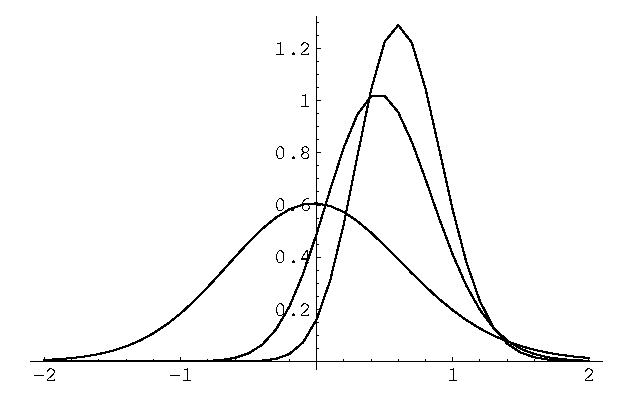
\includegraphics[width=3in]{2007514_1998carlin_standardized_cumulative_likelihood.eps}
\caption{Cumulative marginal likelihood at monitoring dates 1/15/91, 7/31/91, and 12/31/91}
\label{fig:1998carlin_marg}
\end{figure}

\bibliographystyle{plain}
\bibliography{mybib.bib}

\end{document}
